% !TEX root =  paper.tex
\section{Evaluation}
\label{sec:data_eval}
As of writing this paper, there are 654 registered players. In addition, we collected 129,906 events which contains 96,892 gesture events.

\subsection{Method}
We distributed the DigiTaps game to the Apple App Store. We would like the game to be exposed to a large group of users both sighted and unsighted. We also publicized the game through mailing lists that are actively used in the braille community. 

\subsection{Demographics}
The following are the result of the 6 demographics questions we asked.
\begin{enumerate}
  \item \textbf{How old are you?} \\
  47.71\% of the 654 players are under the age of 25 (see figure \ref{age}) with players aged between 18 and 25 years old is the largest population in this group. Since DigiTaps is a game, this result is not surprising. People at a younger age may want to try out the game more than the older people.

\begin{figure}[!htbp]
  \centering
  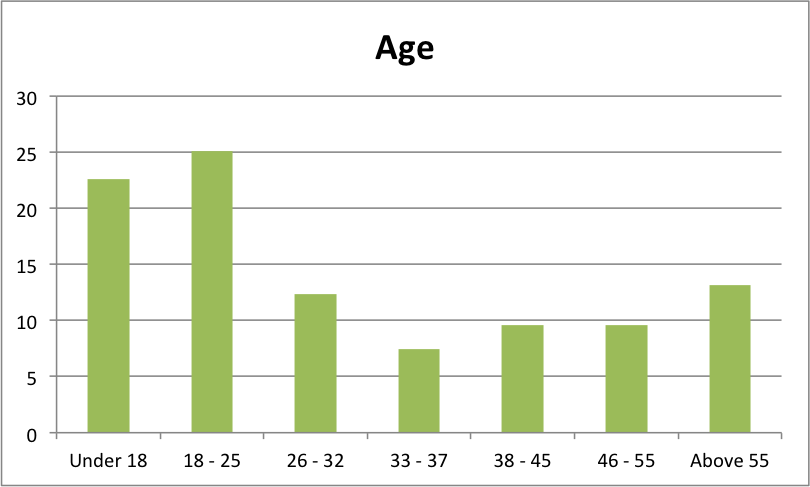
\includegraphics[width=1.0\textwidth]{figures/chart-age.png}
  \caption{Age among all the players.}
  \label{age}
  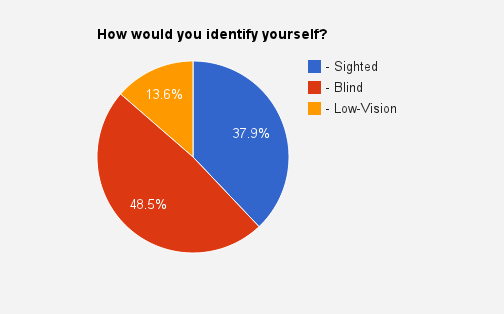
\includegraphics[width=1.0\textwidth]{figures/chart-identity.png}
  \caption{Players' identification among all the players}
  \label{identity}
\end{figure}

  \item \textbf{What is your gender?} \\
  The genders are split almost evenly between male and female. Male accounts for 48.01\% and female accounts for 51.99\% of all the DigiTaps players.

  \item \textbf{How would you identify yourself?} \\
  We advertised DigiTaps through several blind organizations' mailing lists. It is not surprising that 48.5\% of the 654 players indentified themselves as blind (see figure \ref{identity}). Sighted players contributes 37.9\% of all the players.

\begin{figure}[!htbp]
  \centering
  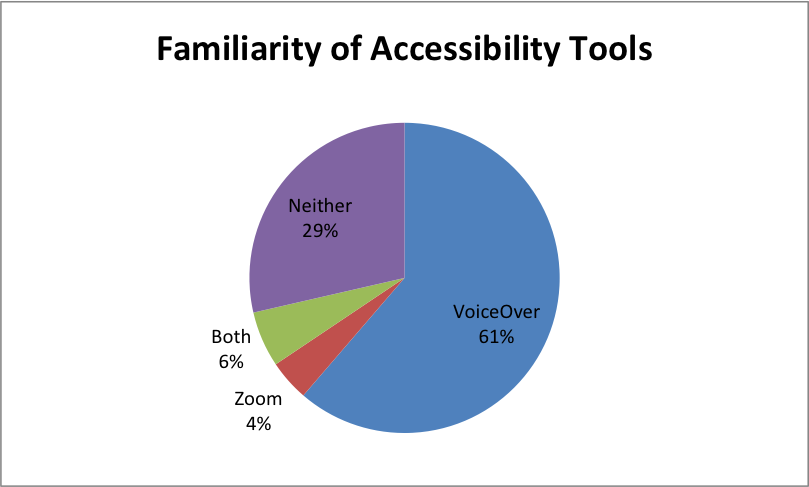
\includegraphics[width=1.0\textwidth]{figures/chart-tools.png}
  \caption{Accessibility tool usage among all the players.}
  \label{tool}
  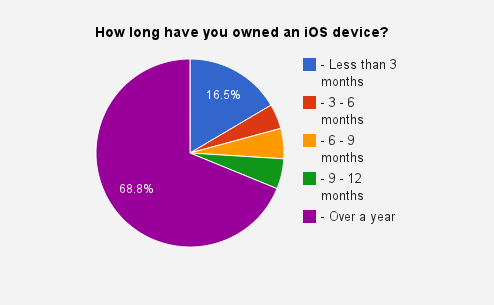
\includegraphics[width=1.0\textwidth]{figures/chart-own.png}
  \caption{How long the player possessed his device among all the players}
  \label{own}
\end{figure}

  \item \textbf{Do you use any accessibility tool on a daily basis?} \\
  Since 48.5\% of the players identified themselves as blind, it is not surprising that the majority of the players uses VoiceOver on a daily basis. However, there are 61.3\% players who use VoiceOver regularly, which is more than 10\% greater than the number of blind players (see figure \ref{tool}. One possible explanation is  13.6\% of the players identified themselves as having low-vision. Low-vision and blind players combined are 62.1\% of all the players.

  \item \textbf{How long have you owned an iOS device?} \\
  We also asked how long that they owned the device, so we can measure their fluency with the platform. The majority, 68.8\%, of the players own their device for over a year (see figure \ref{own}). The second largest population is the players that owns the phone less than 3 months.

\end{enumerate}

\par
From all the players who played the DigiTaps game, we select the top 6 players ranked by the amount of numbers the entered. We evaluate the performance of each player on different type of gestures by measuring the accuracy and the speed when the player enter the numbers. We will identify each of the player as P1 to P6, respectively.

\subsection{Results}
Even though there is some game play that can do some data analysis on the two gestures, the number of taps of each method varies significantly. For example, P3 entered only 7 numbers using Cappuccino while entered 392 number using Espresso. Likewise, P6 did not enter any number using the Cappuccino method. As a result, some results of some players is significantly different from other players and strongly influenced our results.

\subsubsection{Overall Accuracy}
By using the Espresso method, P1 entered 87\% of the numbers correctly and was the most accurate player among the six players. By contrast, the least accurate player, P4, entered 75\% of the numbers correctly. On the other hand, P1 was also the player who entered the number most accurately using the Cappuccino method. P1 achieved an accuracy rate of 90\% over 962 digits.

\subsubsection{Overall Speed}
P4 entered the numbers the fastest at the rate of 0.48 digits per second ($SD=0.16$) with an accuracy of 75\% using the Espresso method. P2 was slowest among all the six players with 0.32 digits per second ($SD=0.13$). In comparison, P5 achieved the highest entry rate of 0.52 digits per second ($SD=0.09$) using the Cappuccino method while the player is still 87\% accurate. P2 was also the slowest using the Cappuccino method. P2 entered the numbers at the rate of 0.31 digits per second ($SD=0.13$).

\subsubsection{Accuracy Development}
We use the same subset of players, P1 through P6, to examine how the players improve their accuracy and entry rate over time. To mimic one session in the lab study presented in \cite{Azenkot:2013}, the numbers that a player entered are divided into six equal groups. In addition to the six groups, there is one more group that contains the rest of the numbers that cannot fit into the first six groups.
\par
In Espresso, players started with accuracies ranging from 70\% to 89\%. As the players progressed, they did not necessary improve their accuracies between sessions. For example, P4's accuracy dropped by 45\% as the player progressed from session 2 to session 3. However, as they progressed to further sessions, their accuracies improved. At the end of the sixth session, all of the players improved their accuracies (figure \ref{esp_accuracy_overtime}). We also observed the same trend in the Cappuccino method (figure \ref{cap_accuracy_overtime}).

\begin{figure}[!htbp]
  \centering
  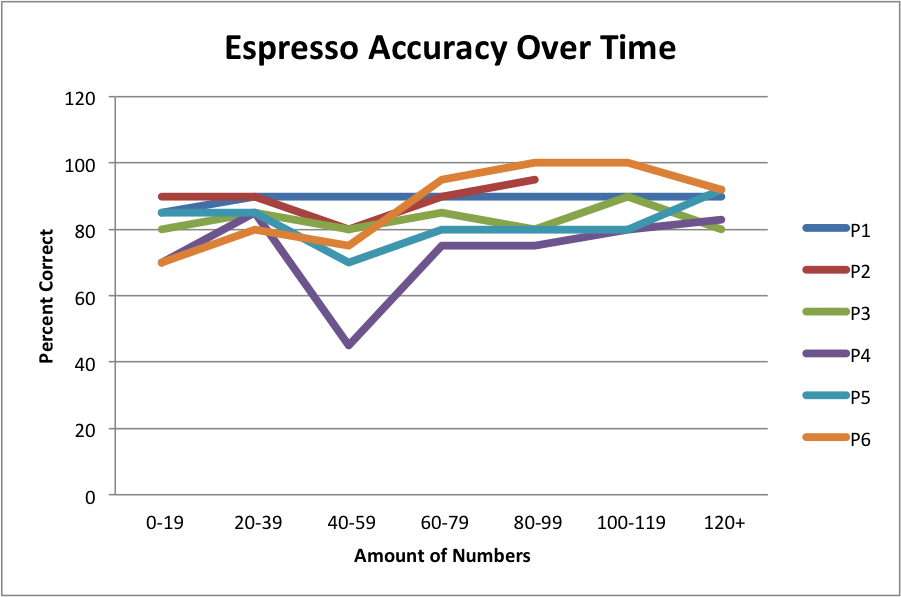
\includegraphics[width=1.0\textwidth]{figures/esp_acc_overtime.png}
  \caption{Breakdown of the accuracy per every 20 numbers for players using the Espresso method}
  \label{esp_accuracy_overtime}
  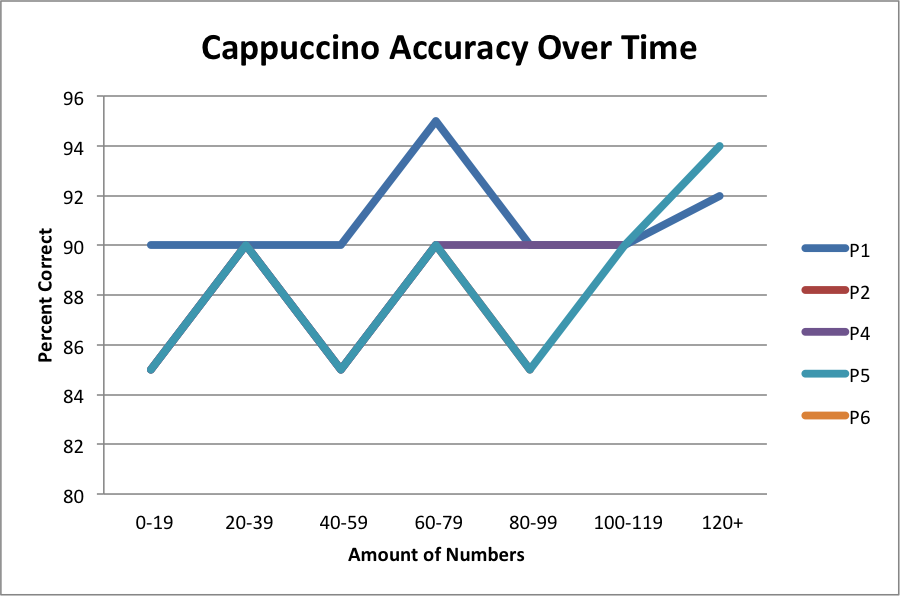
\includegraphics[width=1.0\textwidth]{figures/cap_accuracy_overtime.png}
  \caption{Accuracy per every 20 numbers for players using the Espresso method}
  \label{cap_accuracy_overtime}
\end{figure}

\subsubsection{Speed Development}
In Espresso, Players started with entry rates ranging from 0.20 to 0.55 digits per second. As the players progressed through the sessions, most players gradually improved their entry rates and achieved at least a 40\% increase. However, we observed a different result for P4. Surprisingly, the number entry rate of P4 declined at the end of the sixth session (figure \ref{esp_speed_overtime}). The players' number entry rates improvement is not as clear in the Cappuccino method. There are marginal improvements to the number entry rates of the players. However, all the players improved their number entry rates at the end of the sixth session. The seventh session may contain few numbers and that can strongly influence the entry rate for the session (figure \ref{cap_speed_overtime}).

\begin{figure}[!htbp]
  \centering
  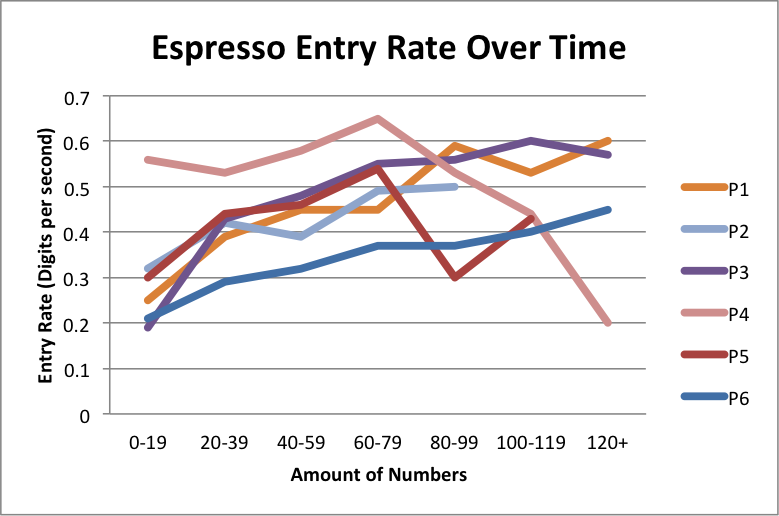
\includegraphics[width=1.0\textwidth]{figures/esp_speed_overtime.png}
  \caption{Speed per every 20 numbers for players using the Espresso method}
  \label{esp_speed_overtime}
  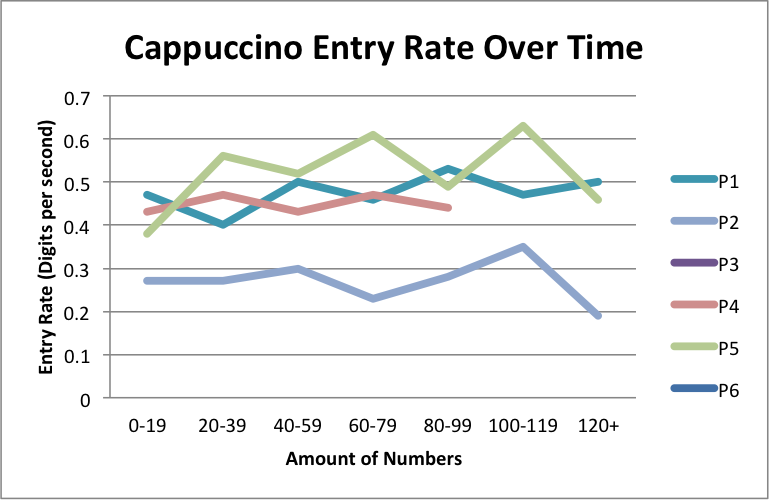
\includegraphics[width=1.0\textwidth]{figures/cap_speed_overtime.png}
  \caption{Speed per every 20 numbers for players using the Espresso method}
  \label{cap_speed_overtime}
\end{figure}

\subsubsection{Game Trends}
Players played the first few levels more often than the later levels. On level 1, The 6 players entered more than 200 numbers using the Cappuccino method and almost 150 numbers using the Espresso method. However, the amount of numbers entered decreased by 62.5\% and 66.7\% in the Cappuccino method and the Espresso method, respectively. The amount of numbers entered continued to decline in the subsequent levels (figure \ref{levels-played}).
\begin{figure}[!htbp]
  \centering
  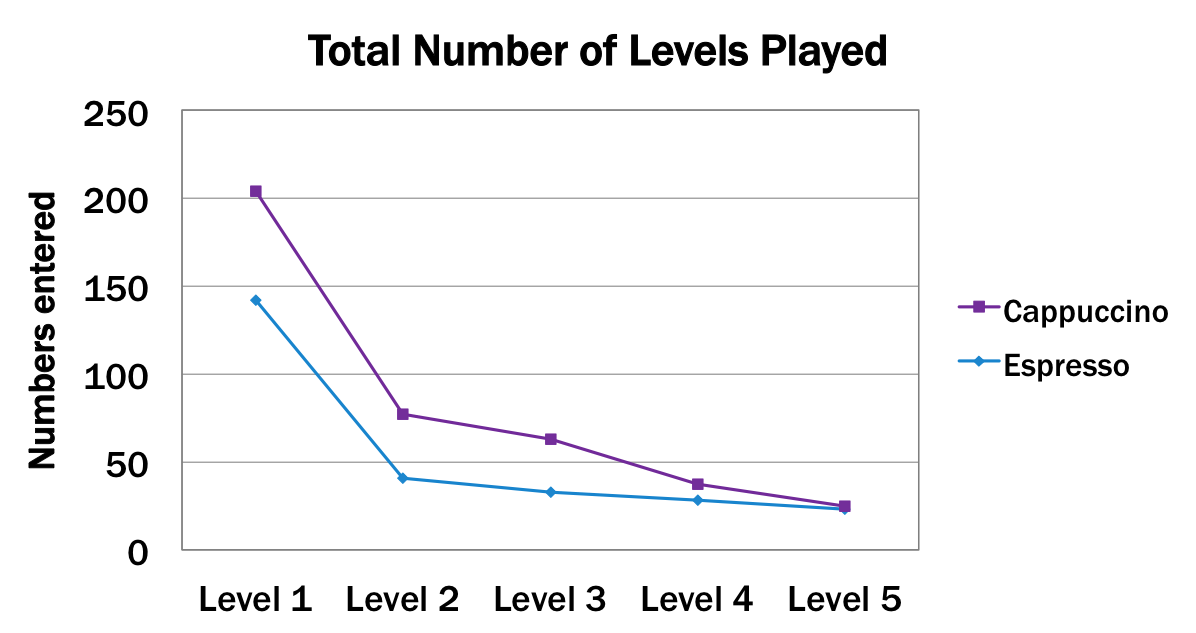
\includegraphics[width=1.0\textwidth]{figures/levels-played.png}
  \caption{Amount of numbers entered in each level.}
  \label{levels-played}
\end{figure}
